	\pagestyle{fancy}
	\section{Berechnungsmodell}\label{sec:Berechnungsmodell}
	\subsection{Potentielle und kinetische Energie eines Balkens}\label{sec:E-Berechnung}
	
	In dieser Arbeit wird der Frässchaft als ein einseitig eingespannter und ungedämpfter Balken mit Exzentrizitätsfehler modelliert. Die potentielle Energie in Abhängigkeit der Green-Lagrange-Dehnung $ \varepsilon_{GL} $, der Durchbiegungen $ v $ und $ w $ sowie die Verdrehung $ \phi $ lautet nach \cite{gross2004technische}
	
	\begin{equation}\label{equ:Epot}
	E_{pot} = \dfrac{EA}{2} \underset{(L)}{\int} \varepsilon_{GL}^{2} \ \dx + \dfrac{EI}{2} \underset{(L)}{\int} w_{xx}^{2} \ \dx + \dfrac{EI}{2} \underset{(L)}{\int} w_{xx}^{2} \ \dx + \dfrac{GI_{t}}{2} \underset{(L)}{\int} \phi_{xx}^{2} \ \dx \ .
	\end{equation}
	
	Die kinetische Energie wird durch den Exzentrizitätsfehler $ e $ und die Winkelgeschwindigkeit $ \Omega $ beeinflusst. Wie Abbildung \ref{fig:Ekin-Rotation} zeigt,
	lautet der Ortsvektor eines beliebigen Punkts des Balkens im $ X_{1}Y_{1}Z_{1} $-Koordinatensystem nach \cite{wauer2014kontinuumsschwingungen}
	
	\begin{equation}\label{equ:Vektor-(1)rp}
	_{\left( 1\right) }\vec{r}_{p} = 
	\left[
	\begin{array}{l}
	X+u-Yv_{x}-Zw_{x}\\
	Y+v-Z\phi\\
	Z+w+Y\phi
	\end{array}
	\right] \ .  
	\end{equation}
	
	\begin{figure}[H]
		\centering
		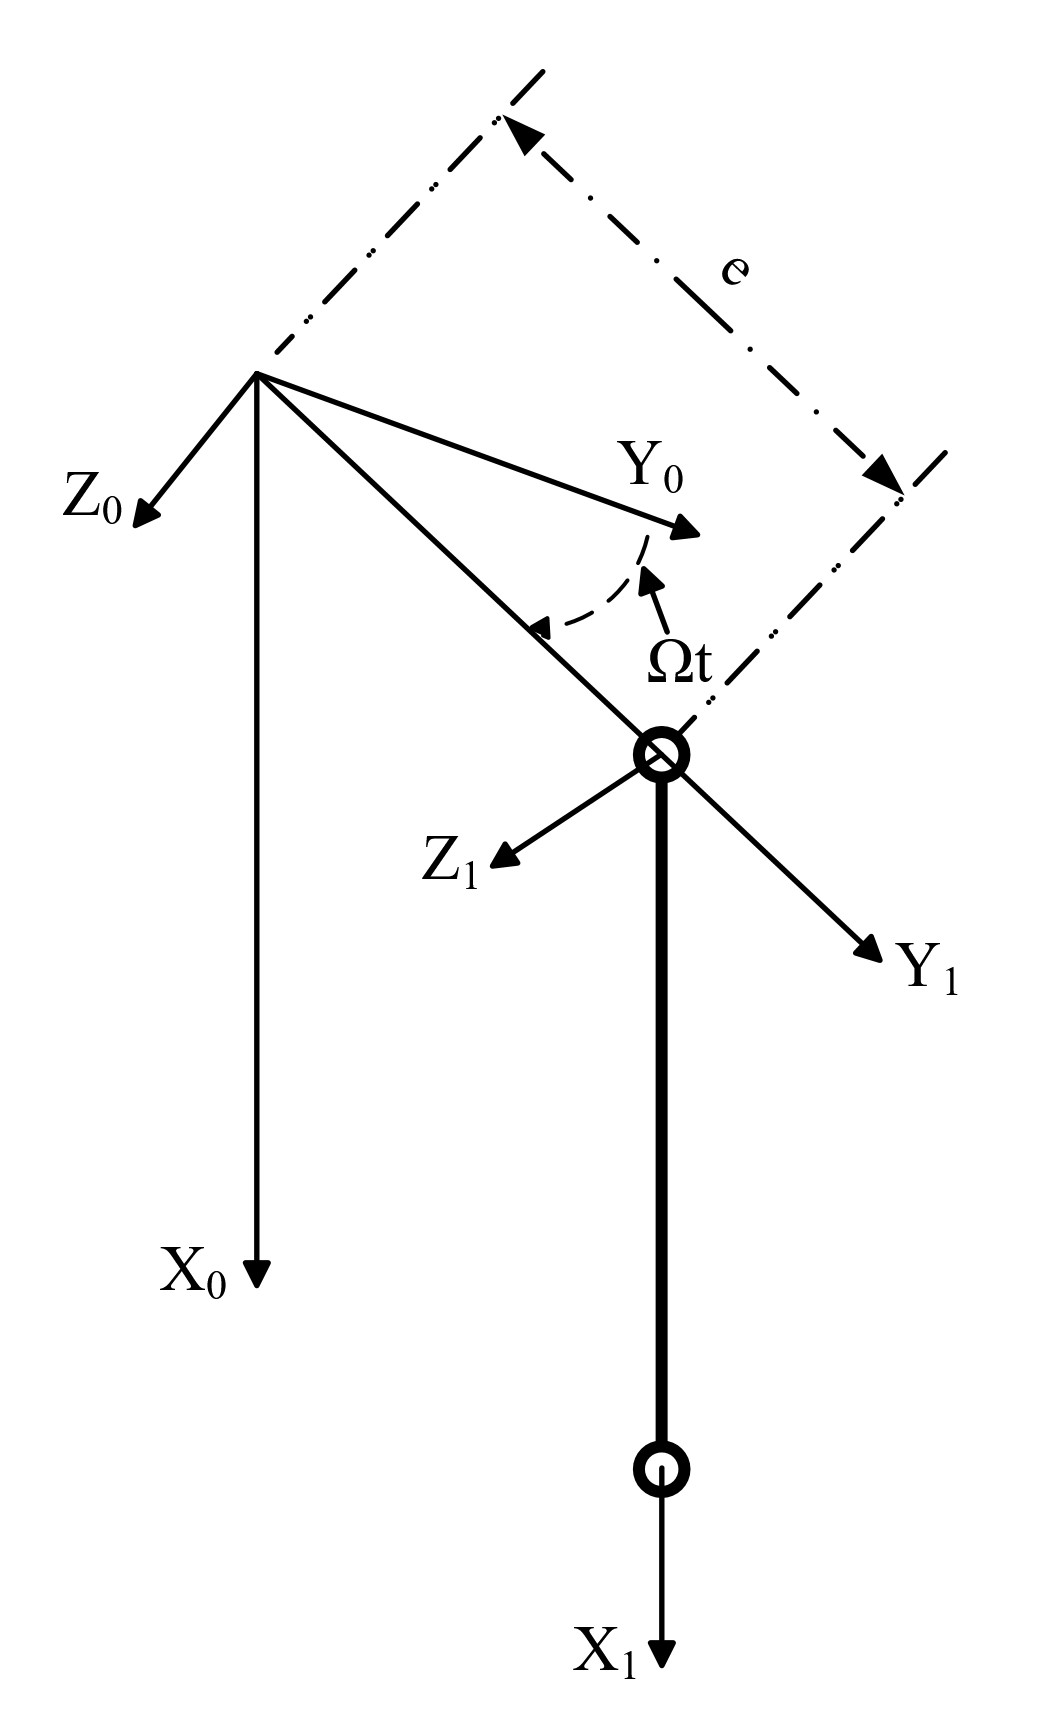
\includegraphics[width=0.45\linewidth, height=0.45\textheight]{Berechnungsmodell/Ekin_Rotation}
		\caption{Balken mit Rotation und Exzentrizitätsfehler.}
		\label{fig:Ekin-Rotation}
	\end{figure}
	
	
	Mit der Rotationsmatrix $ ^{01}\mathbf{R} $ und dem Translationsvektor $ _{(0)}\vec{r}_{12} $ wird der Ortsvektor eines beliebigen Punktes des Balkens im Koordinate $ X_{0}Y_{0}Z_{0} $-Korrdinatensystem mit \cite{heimann2015mechatronik} :
	
	\begin{equation}\label{equ:Vektor-(0)rp}
	%\setlength{\arraycolsep}{2pt}
	_{\left( 0\right) }\vec{r}_{p} = _{\left( 0\right) }\vec{r}_{12} + ^{01}\mathbf{R}\cdot_{\left( 1\right) }\vec{r}_{p} =
	\left[ 
	\begin{array}{c}
	0\\
	e\cdot\cos \Omega t\\
	e\cdot\sin \Omega t
	\end{array}
	\right] +
	\left[  
	\begin{array}{ccc}
	1 & 0 & 0\\
	0 & \cos\Omega t & -\sin\Omega t\\
	0 & \sin\Omega t & \cos\Omega t
	\end{array} 
	\right] \cdot
	\left[
	\begin{array}{l}
	X+u-Yv_{x}-Zw_{x}\\
	Y+v-Z\phi\\
	Z+w+Y\phi
	\end{array}
	\right] 
	\end{equation}
	
	angegeben. Damit ergibt sich die kinetische Energie des Balkens nach \cite{gross2004technische} zu
	
	\begin{equation}\label{equ:Ekin}
	E_{kin} = \dfrac{\rho}{2} \underset{(V)}{\int} \left( \dfrac{\partial _{\left( 0\right) }\vec{r}_{p}}{\partial t} \right)^{2} \ \mathrm{d}V
	= \dfrac{\rho}{2} \underset{(L)}{\int} \underset{(A)}{\int} \left( _{\left( 0\right) }\vec{v}_{p}\right) ^{2} \ \mathrm{d}A \ \dx \ .
	\end{equation}
	
	Mit den folgenden Integralen
	
	\begin{equation}\label{equ:Ekin-Ansatz}
	\setlength{\arraycolsep}{8pt}
	\renewcommand{\arraystretch}{1.3}
	\begin{array}{ll}
	\underset{(A)}{\int} 1 \ \mathrm{d}A = A & \underset{(A)}{\int} Y \ \mathrm{d}A = \underset{(A)}{\int} Z \ \mathrm{d}A = 0\\
	\underset{(A)}{\int} YZ \ \mathrm{d}A =0 & \underset{(A)}{\int} Y^{2} \ \mathrm{d}A = \underset{(A)}{\int} Z^{2} \ \mathrm{d}A = I
	\end{array}
	\end{equation}
	
	lautet die modifizierte kinetische Energie
	\begin{equation}\label{equ:Mod.-Ekin}
	\begin{aligned}
	E_{kin} = \ & \dfrac{\rho A}{2} \underset{(L)}{\int} u_{t}^{2}+e^{2}\Omega^{2}+v^{2}\Omega^{2}+v_{t}^{2}+w^{2}\Omega^{2}+w_{t}^{2}+2ev\Omega^{2}+2ew_{t}\Omega+2vw_{t}\Omega-2v_{t}w\Omega \dx\\
	& +\dfrac{\rho I}{2} \underset{(L)}{\int} v_{xt}^{2}+w_{xt}^{2}+2\Omega^{2}+2\phi^{2}\Omega^{2}+2\phi_{t}^{2}+4\phi_{t}\Omega \dx \ .
	\end{aligned}
	\end{equation}
	
	
	Für die Lösung des Eigenwertproblems des drehenden nichtlinearen Balkens mit Exzentrizitätsfehler wird ein dreidimensionales finites Balkenelement verwendet, wie Bild \ref{fig:2-Knote-Element-Koordinate} gezeigt. Für die Integration und Differentiation der Elemente wird die lokale Koordinate $\xi$ von -1 bis +1 definiert. Die globale Länge eines Elements ist mit $ l_{e} $ gegeben. Der Zusammenhang zwischen lokaler und globaler Koordinate lautet
	\begin{equation}\label{equ:Lokal-zu-global}
	\left. 
	\begin{array}{l}
	\xi (x) = a_{0} + a_{1}x\\
	\xi (x=0) \overset{!}{=} -1\\
	\xi (x=l_{e})  \overset{!}{=} 1
	\end{array} 
	\right\rbrace \Rightarrow 
	\xi = -1 + \frac{2}{l_{e}}x
	\Rightarrow
	\frac{\partial \xi}{\partial x} = \frac{2}{l_{e}}.
	\end{equation}
	
	\subsection{Das dreidimensionale zweiknotige Balkenelement }\label{sec:3D-2.Knote-Balkenelment}
	Bei diesem Element werden die Längsverschiebung $ u $, die Durchbiegungen $ v $ und $ w $ sowie die Verdrehung $ \phi $ durch lineare oder kubische Ansatzfunktionen beschrieben. Für die Längsverschiebung $ u(\xi) $ eines Elements soll der lineare Ansatz
	
	\begin{equation}\label{equ:Linear-Einsatz}
	u(\xi)=a_{0}+a_{1}\xi \ ; \ u(-1) \overset{!}{=} u_{1} \ ; \  u(1) \overset{!}{=} u_{2}
	\end{equation}
	
	verwendet werden. Damit ergibt sich die Längsverschiebung in Vektor-Matrix Schreibweise zu
	
	\begin{equation}\label{equ:Linear-Einsatz-Algebra}
	u(\xi,t) = \vec{N}_{u}(\xi) \vec{u}(t) =
	\left[ \begin{array}{cc}
	\frac{1}{2} - \frac{\xi}{2} & \frac{1}{2} + \frac{\xi}{2}
	\end{array} \right]	
	\left[ 
	\begin{array}{c}
	u_{1}\\
	u_{2}
	\end{array} 
	\right] .
	\end{equation}
	
	Für die Verdrehung $ \phi $ wird auch ein linearer Ansatz analog zur Längsverschiebung verwendet. Deshalb ist die Vektor-Matrix Schreibweise auch identisch. Im Gegensatz dazu wird ein kubischer Ansatz für die Durchbiegung $ w $ mit
	
	\begin{equation}\label{equ:Kubik-Ansatz}
	\begin{array}{c}
	w(\xi) = a_{0} + a_{1}\xi + a_{2}\xi^{2} + a_{3}\xi^{3}\\
	w(-1)\overset{!}{=}w_{1} \ ; \ w_{,\xi}(-1)\overset{!}{=}\varphi_{1} \ ; \ w(+1)\overset{!}{=}w_{2} \ ; \ w_{,\xi}(+1)\overset{!}{=}\varphi_{2} \ .
	\end{array}
	\end{equation}
	
	definiert. Damit kann die Durchbiegung in Vektor-Matrix-Schreibweise mit
	
	\begin{equation}\label{equ:Kubik-Ansatz-Algebra}
	\renewcommand\arraystretch{1.5}
	w(\xi,t) = 
	\vec{N}_{w}(\xi) \vec{w}(t)
	=
	\left[ 
	\begin{array}{c}
	-\frac{1}{16}+\frac{\xi}{16}+\frac{9\xi^{2}}{16}-\frac{9\xi^{3}}{16}\\
	\frac{9}{16}-\frac{27\xi}{16}-\frac{9\xi^{2}}{16}+\frac{27\xi^{3}}{16}\\
	\frac{9}{16}+\frac{27\xi}{16}-\frac{9\xi^{2}}{16}-\frac{27\xi^{3}}{16}\\
	-\frac{1}{16}-\frac{\xi}{16}+\frac{9\xi^{2}}{16}+\frac{9\xi^{3}}{16}
	\end{array}
	\right]^{\mathrm{T}} \cdot
	\left[ 
	\begin{array}{c}
	w_{1}\\
	\varphi_{1}\\
	w_{2}\\
	\varphi_{2}
	\end{array}
	\right]	
	\end{equation}
	
	angegeben werden. Darin kennzeichnen $\varphi_{i}$ die Biegewinkel der Knoten. Für die Durchbiegung $ v $ und dem dazugehörigen Biegewinkel $ \psi $ wird ein identischer Ansatz zu $w$ und $\varphi$ benutzt. Durch die oben genanten Ansätze lautet der Vektor der Knotenvariablen $ \vec{x} $
	
	\begin{equation}\label{equ:Knotenverformung-P}
	\vec{x} = \left[ \left. \ u_{1} \ \right|  \  w_{1} \ \left| \  \varphi_{1} \ \right| \  v_{1} \ \left| \ \psi_{1} \ \right| \ \phi_{1} \ \left| \  u_{2} \ \right| \ w_{2} \ \left| \ \varphi_{2} \ \right|  \  v_{2} \ \left| \  \psi_{2} \ \right| \  \phi_{2} \   \right]^{\mathrm{T}} .
	\end{equation}
	Die Verschiebungen im Element werden durch den Vektor $ \vec{x}_{e}=[ \,u \, | \, w \, | \, v \, | \, \phi \, ] $ beschrieben und ergeben sich nach \cite{steinke2015finite} zu
	
	\begin{equation}\label{equ:Verschiebungen-P-Element}
	\begin{aligned}
	\vec{x}_{e} & =\vec{N}\vec{x} = 
	\left[ 
	\left. \ \vec{N}^{u} \ \right|  \  \vec{N}^{w} \ \left| \  \vec{N}^{v}  \ \right| \ \vec{N}^{\phi} \ \right]^{\mathrm{T}} \vec{x}\\[2mm]
	&= 
	\left[
	\setlength{\arraycolsep}{4pt}
	\begin{array}{llllllllllll} 
	N_{u1} & 0        & 0        & 0        & 0        & 0          & N_{u2} & 0        & 0        & 0        & 0        & 0\\
	0      & N_{w1}   & N_{w2}   & 0        & 0        & 0          & 0      & N_{w3}   & N_{w4}   & 0        & 0        & 0\\
	0      & 0        & 0        & N_{v1}   & N_{v2}   & 0          & 0      & 0        & 0        & N_{v3}   & N_{v4}   & 0\\
	0      & 0        & 0        & 0        & 0        & N_{\phi 1} & 0      & 0        & 0        & 0        & 0        & N_{\phi 1}\\ 
	\end{array}
	\right] \vec{x} \ .
	\end{aligned}
	\end{equation}
	
	Die Ableitung der Formfunktionen $ \vec{N}_{x} $ nach der globalen Variable $ x $ kann durch den Zusammenhang (\ref{equ:Lokal-zu-global}) 
	\begin{equation}\label{equ:X-Ableitung-Formfunktion}
	\vec{N}_{x}(\xi) = \dfrac{\partial \vec{N}(\xi)}{\partial \xi} \cdot \dfrac{\partial \xi}{\partial x} = \dfrac{\partial \vec{N}(\xi)}{\partial \xi} \cdot \dfrac{2}{l_{e}} 
	\end{equation}
	mit berechnet werden
	
	\subsection{Variationsformulierung}\label{sec:Matrizenrechnung}
	In Kapitel (\ref{sec:E-Berechnung}) wurden die kinetische und potenzielle Energie (Gleichungen  \ref{equ:Mod.-Ekin} und \ref{equ:Epot}) schon berechnet. Damit lässt sich das Prinzip von Hamilton (Gleichung \ref{equ:Hamilton})	auswerten. Mit der Annahme, dass für die virtuelle Arbeit der potentiallosen Kräfte $ \delta W=0$ gilt, vereinfacht sich Gleichung \eqref{equ:Hamilton} zu
	
	\begin{equation}\label{equ:Hamilton-mit-Energie-Mod.}
	\int_{t_{1}}^{t_{2}} \delta E_{kin} \, \dt  - \int_{t_{1}}^{t_{2}} \delta E_{pot} \dt = 0.
	\end{equation}
	
	Nach der Variation sowie partiellen Integration ergibt sich die kinetische Energie zu
	\begin{equation}\label{equ:Hamilton-Variation-Partiell-Mod.}
	\begin{aligned}
	\delta E_{kin} = & \rho A \int_{t_{1}}^{t_{2}} \underset{(L)}{\int} -u_{tt}\delta u - v_{tt}\delta v - w_{tt}\delta w - 2v_{t}\Omega \delta w + 2w_{t} \Omega \delta v + v\Omega^{2}\delta v + w\Omega^{2}\delta w  \dx  \dt \\
	& + \rho I \int_{t_{1}}^{t_{2}} \underset{(L)}{\int} -v_{xtt}\delta v_{x} - w_{xtt}\delta w_{x} - 2\phi_{tt}\delta \phi \dx \dt + 2\phi \Omega^{2}\delta \phi  \\
	& + \rho A \int_{t_{1}}^{t_{2}} \underset{(L)}{\int} e\Omega^{2}\delta v \dx \dt
	\end{aligned}
	\end{equation}
	
	und die potenzielle Energie zu
	
	\begin{equation}\label{equ:Epot-mit-Variation}
	\begin{aligned}
	\delta E_{pot} = & \dfrac{EA}{2} \underset{(L)}{\int} \left[ \left( 2u_{x}+3u_{x}^{2}+v_{x}^{2}+w_{x}^{2}+u_{x}^{3}+u_{x}v_{x}^{2}+u_{x}w_{x}^{2}\right) \delta u_{x} \right. \\[1mm]
	& + \left( 2v_{x}u_{x}+v_{x}u_{x}^{2}+v_{x}^{3}+v_{x}w_{x}^{2} \right) \delta v_{x} + \left. \left( 2w_{x}u_{x}+w_{x}u_{x}^{2}+w_{x}v_{x}^{2}+w_{x}^{2} \right) \delta w_{x} \right] \dx  \\[2mm]
	& + EI \underset{(L)}{\int} v_{xx}\delta v_{xx} + w_{xx}\delta w_{xx} \, \dx + EI_{t} \underset{(L)}{\int} \phi_{x}\delta \phi_{x} \, \dx \ .
	\end{aligned}  
	\end{equation}
	
	Wegen der Nichtlinearität wird die variierte potenzielle Energie durch eine Taylorreihe linearisiert. Die linearisierte potenzielle Energie lautet
	\begin{equation}\label{equ:Epot-mit-Taylor-Variation}
	\begin{aligned}
	\Delta \delta E_{pot} & = \dfrac{\partial \delta E_{pot}}{\partial u_{x}}\Delta u_{x} + \dfrac{\partial \delta E_{pot}}{\partial v_{x}}\Delta v_{x} +\dfrac{\partial \delta E_{pot}}{\partial w_{x}}\Delta w_{x} +\dfrac{\partial \delta E_{pot}}{\partial v_{xx}}\Delta v_{xx} +\dfrac{\partial \delta E_{pot}}{\partial w_{xx}}\Delta w_{xx} + \dfrac{\partial \delta E_{pot}}{\partial \phi_{x}}\Delta \phi_{x} \\[2mm]
	& = EA \underset{(L)}{\int} \left[ \left( 1+3u_{x}+\dfrac{3}{2}u_{x}^{2}+\dfrac{1}{2}v_{x}^{2}+\dfrac{1}{2}w_{x}^{2} \right) \Delta u_{x} + \left( v_{x}+v_{x}u_{x} \right) \Delta v_{x} + \left( w_{x}+w_{x}u_{x} \right) \Delta w_{x} \right] \delta u_{x} \dx \\[2mm]
	& \quad + EA \underset{(L)}{\int} \left[ \left( v_{x}+v_{x}u_{x} \right) \Delta u_{x} + \left( u_{x}+\dfrac{1}{2}u_{x}^{2}+\dfrac{3}{2}v_{x}^{2}+\dfrac{1}{2}w_{x}^{2} \right) \Delta v_{x} + \left( v_{x}w_{x} \right) \Delta w_{x} \right] \delta v_{x} \dx \\[2mm]
	& \quad + EA \underset{(L)}{\int} \left[ \left( w_{x}+w_{x}u_{x} \right) \Delta u_{x} + \left( v_{x}w_{x} \right) \Delta v_{x} + \left( u_{x}+\dfrac{1}{2}u_{x}^{2}+\dfrac{1}{2}v_{x}^{2}+\dfrac{3}{2}w_{x}^{2} \right) \Delta w_{x} \right] \delta w_{x} \dx .
	\end{aligned}
	\end{equation}
	
	Die linearisierte potenzielle Energie wird in Gleichung (\ref{equ:Hamilton-mit-Energie-Mod.}) eingesetzt, wodurch
	
	\begin{equation}\label{equ:Hamilton-mit-lin.Energie-Mod.}
	\int_{t_{1}}^{t_{2}} \delta E_{kin} \, \dt  - \int_{t_{1}}^{t_{2}} \Delta\delta E_{pot} \dt = 0
	\end{equation}
	gilt. 
	
	
	\subsection{Diskretisierung}
	Die linearisierte Variationsformulierung aus dem vorherigen Abschnitt wird mit dem FE-Ansatz aus Gleichung \eqref{equ:Verschiebungen-P-Element} diskretisiert. Damit kann die diskretiserte schwache Formulierung der Bewegungsdifferentialgleichung mit
	
	\begin{equation}\label{equ:Schwache-Formulierung-Bewegung-Ggl}
	\begin{aligned}
	0= \ & \rho A \int_{t_{1}}^{t_{2}}\underset{(L)}{\int} [\vec{N}^{u}]^{\mathrm{T}}\vec{N}^{u}\vec{u}_{tt}\delta \vec{u} \, + \,  [\vec{N}^{v}]^{\mathrm{T}}\vec{N}^{v}\vec{v}_{tt}\delta \vec{v} \, + \, [\vec{N}^{w}]^{\mathrm{T}}\vec{N}^{w}\vec{w}_{tt}\delta \vec{w} \, + \, 2\Omega[\vec{N}^{v}]^{\mathrm{T}}\vec{N}^{w}\vec{v}_{t}\delta \vec{w} \\[3mm]
	& - \ 2\Omega[\vec{N}^{w}]^{\mathrm{T}}\vec{N}^{v}\vec{w}_{t}\delta \vec{v} \ - \ \Omega^{2}[\vec{N}^{v}]^{\mathrm{T}}\vec{N}^{v}\vec{v}\delta \vec{v} \ - \ \Omega^{2}[\vec{N}^{w}]^{\mathrm{T}}\vec{N}^{w}\vec{w}\delta \vec{w} \, \dx \dt\\[3mm]
	& + \ \rho I \int_{t_{1}}^{t_{2}}\underset{(L)}{\int} [\vec{N}_{x}^{v}]^{\mathrm{T}}\vec{N}_{x}^{v}\vec{v}_{tt}\delta \vec{v} \ + \ [\vec{N}_{x}^{w}]^{\mathrm{T}}\vec{N}_{x}^{w}\vec{w}_{tt}\delta \vec{w} \ - \ 2\Omega[\vec{N}^{\phi}]^{\mathrm{T}}\vec{N}^{\phi}\vec{\phi}\delta \vec{\phi} \\
	& + \ 2\Omega[\vec{N}^{\phi}]^{\mathrm{T}}\vec{N}^{\phi}\vec{\phi}_{tt}\delta \vec{\phi} \, \dx \dt \ + \ \rho A \int_{t_{1}}^{t_{2}}\underset{(L)}{\int} -e\Omega^{2}[\vec{N}^{v}]^{\mathrm{T}}\delta \vec{v} \, \dx \dt\\[1mm]
	& + \ EA\int_{t_{1}}^{t_{2}}\underset{(L)}{\int} \left[ (1+3u_{x}+\dfrac{3}{2}u_{x}^{2}+\dfrac{1}{2}v_{x}^{2}+\dfrac{1}{2}w_{x}^{2})\vec{N}^{u}_{x}\Delta u \, + \, (v_{x}+v_{x}u_{x})\vec{N}^{v}_{x}\Delta v\right. \\
	& +  \left.  ( w_{x}+w_{x}u_{x} )\vec{N}^{w}_{x}\Delta w\right]^{\mathrm{T}}\vec{N}^{u}_{x} \delta u \, \dx \dt + EA\int_{t_{1}}^{t_{2}}\underset{(L)}{\int} \left[ (u_{x}+\dfrac{1}{2}u_{x}^{2}+\dfrac{3}{2}v_{x}^{2}+\dfrac{1}{2}w_{x}^{2})\vec{N}_{x}^{v}\Delta v \right. \\
	& +  \left. (v_{x}+v_{x}u_{x})\vec{N}_{x}^{u}\Delta u + (v_{x}w_{x})\vec{N}_{x}w\Delta w \right]^{\mathrm{T}} \vec{N}_{x}^{v} \delta v \dx \dt + EA\int_{t_{1}}^{t_{2}}\underset{(L)}{\int} \left[ (w_{x}+w_{x}u_{x})\vec{N}_{x}^{u}\Delta u \right. \\
	& + \left. (v_{x}w_{x})\vec{N}_{x}^{v}\Delta v + (u_{x}+\dfrac{1}{2}u_{x}^{2}+\dfrac{1}{2}v_{x}^{2}+\dfrac{3}{2}w_{x}^{2})\vec{N}_{x}^{w}\Delta w \right]^{\mathrm{T}}\vec{N}_{x}^{w} \delta w \dx \dt .  \\
	\end{aligned}
	\end{equation}
	
	angegeben werden. Die Massenmatrix eines Elements lautet
	
	\begin{equation}\label{equ:Massenmatrix}
	\begin{aligned}
	\mathbf{M}_{e} = & \int_{-1}^{+1} \rho A\left(   [\vec{N}^{u}]^{\mathrm{T}}\vec{N}^{u} + [\vec{N}^{v}]^{\mathrm{T}}\vec{N}^{v} + [\vec{N}^{w}]^{\mathrm{T}}\vec{N}^{w}\right) \\[2mm]
	& + \rho I \left(  [\vec{N}_{x}^{v}]^{\mathrm{T}}\vec{N}_{x}^{v} + [\vec{N}_{x}^{w}]^{\mathrm{T}}\vec{N}_{x}^{w} + 2\Omega[\vec{N}^{\phi}]^{\mathrm{T}}\vec{N}^{\phi}\right)   \dxi,
	\end{aligned}
	\end{equation}
	
	die gyroskopische Matrix
	
	\begin{equation}\label{equ:Gyroskopische-Matrix}
	\mathbf{D}_{e} = \rho A\int_{-1}^{+1} 2\Omega[\vec{N}^{v}]^{\mathrm{T}}\vec{N}^{w} - 2\Omega[\vec{N}^{w}]^{\mathrm{T}}\vec{N}^{v} \dxi
	\end{equation}
	
	und Fliehkraftbelastung
	
	\begin{equation}\label{equ:Fliehkraft}
	\vec{f}_{e} = \rho A\int_{-1}^{+1} -e\Omega^{2}[\vec{N}^{v}]^{\mathrm{T}} \dxi .
	\end{equation}
	
	
	
	Zur Angabe der Steifigkeitsmatrix werden die Ableitungen nach $ \dx $ in $ \mathrm{d}\, \xi $ umgeschrieben mittels
	
	\begin{equation}\label{equ:Zusammenhang-dx-dxi}
	\dfrac{\,\mathrm{d} \, \xi}{\dx}=\dfrac{2}{l_{e}} \Rightarrow \dx=\dfrac{l_{e}}{2}\,\mathrm{d}\, \xi.
	\end{equation}
	
	Damit lautet die Elementsteifigkeitsmatrix
	
	\begin{equation}\label{equ:Steifigkeitsmatrix}
	\begin{aligned}
	\mathbf{K}_{e} = & \ \dfrac{l_{e}}{2} \int_{-1}^{+1} \rho A\left( -\Omega^{2}[\vec{N}^{v}]^{\mathrm{T}}\vec{N}^{v} - \Omega^{2}[\vec{N}^{w}]^{\mathrm{T}}\vec{N}^{w}\right) + \rho I \left( -2\Omega[\vec{N}^{\phi}]^{\mathrm{T}}\vec{N}^{\phi}\right) \\
	& + EA \left\lbrace  \left[ (1+3u_{x}+\dfrac{3}{2}u_{x}^{2}+\dfrac{1}{2}v_{x}^{2}+\dfrac{1}{2}w_{x}^{2})\vec{N}^{u}_{x} + (v_{x}+v_{x}u_{x})\vec{N}^{v}_{x} + (w_{x}+w_{x}u_{x})\vec{N}^{w}_{x}\right]^{\mathrm{T}}\vec{N}^{u}_{x} \right. \\
	& + \left[ (u_{x}+\dfrac{1}{2}u_{x}^{2}+\dfrac{3}{2}v_{x}^{2}+\dfrac{1}{2}w_{x}^{2})\vec{N}_{x}^{v} + (v_{x}+v_{x}u_{x})\vec{N}_{x}^{u} + (v_{x}w_{x})\vec{N}_{x}w \right]^{\mathrm{T}}\vec{N}_{x}^{v}\\
	& + \left. \left[ (w_{x}+w_{x}u_{x})\vec{N}_{x}^{u} + (v_{x}w_{x})\vec{N}_{x}^{v} + (u_{x}+\dfrac{1}{2}u_{x}^{2}+\dfrac{1}{2}v_{x}^{2}+\dfrac{3}{2}w_{x}^{2})\vec{N}_{x}^{w} \right]^{\mathrm{T}}\vec{N}_{x}^{w} \right\rbrace  \ \dxi.
	\end{aligned}
	\end{equation}
	
	Die Größe einer Elementmatrix ist $ 12\times12 $. Für die Elementmassenmatrix werden die Einträge folgendermaßen angegeben
	
	\begin{equation}\label{equ:I.ten-Massenmatrix}
	\renewcommand{\arraystretch}{1.3}
	\mathbf{M}_{ei}=
	\left[ 
	\begin{array}{cccc}
	M_{ei;1,1} & M_{ei;1,2} & \cdots & M_{ei;1,12}\\
	M_{ei;2,1} & M_{ei;2,2} & \cdots & M_{ei;2,12}\\
	\colon     & \colon     & \ddots & \colon\\
	M_{ei;12,1}& M_{ei;12,1}& \cdots & M_{ei;12,12}
	\end{array}
	\right] .
	\end{equation}
	
	Damit kann die Gesamtmassenmatrix nach
	
	\begin{equation}\label{equ:Gesamtmassenmatrix}
	\renewcommand{\arraystretch}{1.4}
	\mathbf{M}=
	\left[ 
	\begin{array}{cccccccc}
	M_{e1;1,1}  & \cdots & M_{e1;1,6}  & M_{e1;1,7}             & \cdots     & M_{e1;1,12}             & 0          &\cdots\\
	\colon      & \ddots & \colon      & \colon                 & \ddots     & \colon                  & \colon     &\cdots\\
	M_{e1;6,1}  & \cdots & M_{e1;6,6}  & M_{e1;6,7}             & \cdots     & M_{e1;6,12}             & 0          &\cdots\\
	M_{e1;7,1}  & \cdots & M_{e1;7,6}  & M_{e1;7,7}+M_{e2;1,1}  & \cdots     & M_{e1;7,12}+M_{e2;1,6}  & M_{e2;1,7} &\cdots\\
	\colon      & \ddots & \colon      & \colon                 & \ddots     & \colon                  & \colon     &\cdots\\
	M_{e1;12,1} & \cdots & M_{e1;12,6} & M_{e1;12,7}+M_{e2;6,1} & \cdots     & M_{e1;12,12}+M_{e2;6,6} & M_{e2;6,7} &\cdots\\
	0           & \cdots & 0           & M_{e2;7,1}             & \cdots     & M_{e2;7,6}              & \ddots     &\cdots\\
	\colon      & \colon & \colon      & \colon                 & \colon     & \colon                  & \colon     &\ddots\\
	\end{array}
	\right] 
	\end{equation}
	
	zusammengebaut werden. Nach gleicher Regel werden auch die Steifigkeitsmatrix und die gyroskopische Matrix des gesamten Systems zusammengebaut. Der gesamte Fliehkraftvektor wird nach 
	
	\begin{equation}\label{equ:Gesamtfliehkraft}
	\vec{f} = \left[ 
	\begin{array}{llllllll}
	f_{e1;1} & \cdots & f_{e1;6} & f_{e1;7}+f_{e2;1} & \cdots & f_{e1;12}+f_{e2;6} & f_{e2;7}+f_{e3;1} & \cdots  
	\end{array} 
	\right]^{\mathrm{T}}
	\end{equation} 
	zusammengebaut. Mit den bereits definierten FE-Ansätzen ergibt sich für statische Probleme  nach Gleichung \ref{equ:Einfach-Bewegung-GL} 
	
	\begin{equation}\label{equ:Einfach-Bewegung-GL-mit-P-F}
	\mathbf{K}\, \vec{x} = \vec{f} \ .
	\end{equation}
	und für dynamische Systeme nach Gleichung \ref{equ:Bewegung-GL}
	
	\begin{equation}\label{equ:Bewegung-GL-mit-Matrizen}
	\mathbf{M}\, \ddot{\vec{x}}+ \mathbf{D}\, \dot{\vec{x}}+ \mathbf{K}\, \vec{x} = \vec{f} \ .
	\end{equation}
	
	\subsection{Zustandsraumdarstellung}
	Durch die Definition der Zustandsgrößen
	
	\begin{equation}\label{equ:Ansatz-in-Systemmatrix}
	\left. 
	\begin{array}{c}
	\vec{z}_{1} = \vec{x} \\
	\vec{z}_{2} = \dot{\vec{x}}
	\end{array}
	\right\rbrace \Rightarrow	
	\begin{array}{l}
	\dot{\vec{z}}_{1} = \vec{z}_{2} \\
	\dot{\vec{z}}_{2} = \ddot{\vec{x}} = - \mathbf{M}^{-1} \cdot \mathbf{K} \cdot \vec{z}_{1} - \mathbf{M}^{-1} \cdot \mathbf{D} \cdot \vec{z}_{2}
	\end{array}
	\end{equation}
	
	kann die Gleichung (\ref{equ:Bewegung-GL-mit-Matrizen}) im Zustandsraum
	
	\begin{equation}\label{equ:1st-Ausgangspunkt}
	\left[ 
	\begin{array}{c}
	\dot{\vec{z}}_{1}\\
	\dot{\vec{z}}_{2}
	\end{array}
	\right] 
	=
	\left[ 
	\begin{array}{cc}
	\mathbf{0}                        & \mathbf{E} \\
	-\mathbf{M}^{-1} \cdot \mathbf{K} & -\mathbf{M}^{-1} \cdot \mathbf{D}
	\end{array}
	\right]
	\cdot
	\left[ 
	\begin{array}{c}
	\vec{z}_{1}\\
	\vec{z}_{2}
	\end{array}
	\right] 
	\end{equation}
	angegeben werden. Es kennzeichnet $\textbf{0}$ die Nullmatrix und $\textbf{E}$ die Einheitsmatrix. Die Eigenfrequenzen der Struktur können durch die Eigenwerte der Systemmatrix
	\begin{equation}\label{equ:Systemmatrix}
	\mathbf{A}
	=
	\left[ 
	\begin{array}{cc}
	\mathbf{0}                        & \mathbf{E} \\
	-\mathbf{M}^{-1} \cdot \mathbf{K} & -\mathbf{M}^{-1} \cdot \mathbf{D}
	\end{array}
	\right]
	\end{equation}
	bestimmt werden.\\
	

	